\chapter{The Lambda Architecture [VI]}
\label{chap:lambda_architecture}

%New terms:
% view
% batch layer
% batch view
% serving layer
% speed layer
% real-time view
% raw data
% immutability

The Lambda architecture is a new solution for generic BigData systems \cite{MarzWarren201401}.
To answer queries it uses both batch and online processing.
It fulfills all requirements that such systems demand, e.g. scalability, extensibility, fault-tolerance, etc.
It provides human fault-tolerance, what is often overlooked in other approaches.
All its components automatically distribute computations across many machines.

%The core purpose of the Lambda architecture is to answer queries, having data, gathered during system's functioning.
%We consider any query as a function of the whole dataset, i.e. taking all available data, system can derive information, that answers specific query.
%The Lambda architecture is also able to answer queries that have not yet arised to the moment of the system's design or deployment.

The Lambda architecture uses both batch and online processing of data to answer queries fast as well as accurate.
It applies batch processing to all data to precompute specific data structures helping to answer queries with low-latency.
It also executes online incremental processing of arriving data, what helps to overcome delay of batch computations.

The Lambda architecture has all properties to be an effective and efficient BigData system.
It is robust and fault-tolerant.
It provides low-latency query answering.
It is scalable, generic and extensible.
It allows to make ad hoc queries, requires minimal maintenance, and is debuggable.

Important aspect of the Lambda architecture, that makes a difference with other approaches, is that human fault-tolerance is inherent.
Human fault-tolerance is a robustness of the system to mistakes in programming code.
This is important issue, because programmers always do mistakes.
As a result, deleting or updating the data in a wrong way is also possible.
The Lambda architecture overcome this issue not allowing to delete or modify so far gathered data.

The Lambda architecture is a distributed system.
Every its part provides this property inherently.
That lets developer to concentrate on the logik and algorithms, instead of thinking about multithreading issues.

\section{General structure}

%System must provide information having gathered data from users and other sources.
%Application of complex algorithms is often necessary.
%Amount of data and rate of its arrival are heavy.
%Those aspects makes system to preprocess indices and aggregations that provide useful information.
%Batch processing is a good solution for that, nevertheless it has drawback - execution time is long.
%Incrementall processing resolves this issue.
%In combination these two approaches allow to design a system, that answers user queries with low latency as well as accurate.

%The purpose of the system is to answer queries having data.
%Let's consider an artificial example.
%Suppose we have a website where people pose programming questions, and other answer them.
%In this case the simplest query to the system is to return list of answers for a particular question post.
%Another query is to find all posts containing given keyword.

%One query is easy to answer, another requires application of complex algorithms.
%It is pretty easy to get list of answers to the question post having its id.
%You simply create hash-table that maps questions' ids to lists of answers' ids.
%Search by keyword, or even phrase search, is much more complex.
%To make it possibe we have to build specific inverted index, and this requires much more time to execute and to programm.
%Let's further assume, that our system has to provide keyword search, using precomputed inverted index. 

%Amount of data gathered with the time, as well as intense of arrival, can be huge.
%Let's consider again our example website.
%Assume that on average every second 5 questions and 20 answers appear.
%Every post is about 100 words, each of about 8 unicode symbols.
%The rate of incoming data is then $25*100*8*2=39$ KB per second.
%It is about 3.2 GB per day.
%This leads our system to be able to process such amount of data efficiently, as well as to rapidly reflect the state of inverted index with newly arrived posts.

Amount of data and complexity of algorithms demand to make computations, useful for fast answering queries, in advance.
The Lambda architecture precomputes specific data structures, that provide data, prepared as much as possible to directly answer specific queries.
We call these data structures \textit{views}\mnote{view}.
They store indices and aggregations of original data.
%In our example we consider inverted index as a view.
%In a query time it provides efficient search of all posts with particular keyword.

There two approaches of preparing views.
The first one is to do it in a batch mode considering all available data for computations.
The second one is to construct views incrementally in the real-time with newly arrived data.
Together these two methods give us an opportunity to answer queries fast and accurate.
Figure~\ref{fig:lambda_architecture} depicts how the Lambda architecture combines batch and incremental processing to answer queries.

The \textit{batch layer} \mnote{batch layer} of the Lambda architecture is responsible for batch processing.
It takes the whole dataset and executes batch computations on it.
Views, that are the result of the batch processing, we call \textit{batch views} \mnote{batch view}. 
This operation is efficient, because all data is at once in disposal.
We can execute any algorithm, and produce any kind of index or aggregation.
It is also easy to programm using such greate batch processing approaches as MapReduce.
This paradighm is inherently distributed and scalable.
%In example with website we would use MapReduce to create inverted index having all posts.
%It requires only several lines of code in the simplest case. 

\begin{figure}
  \centering
  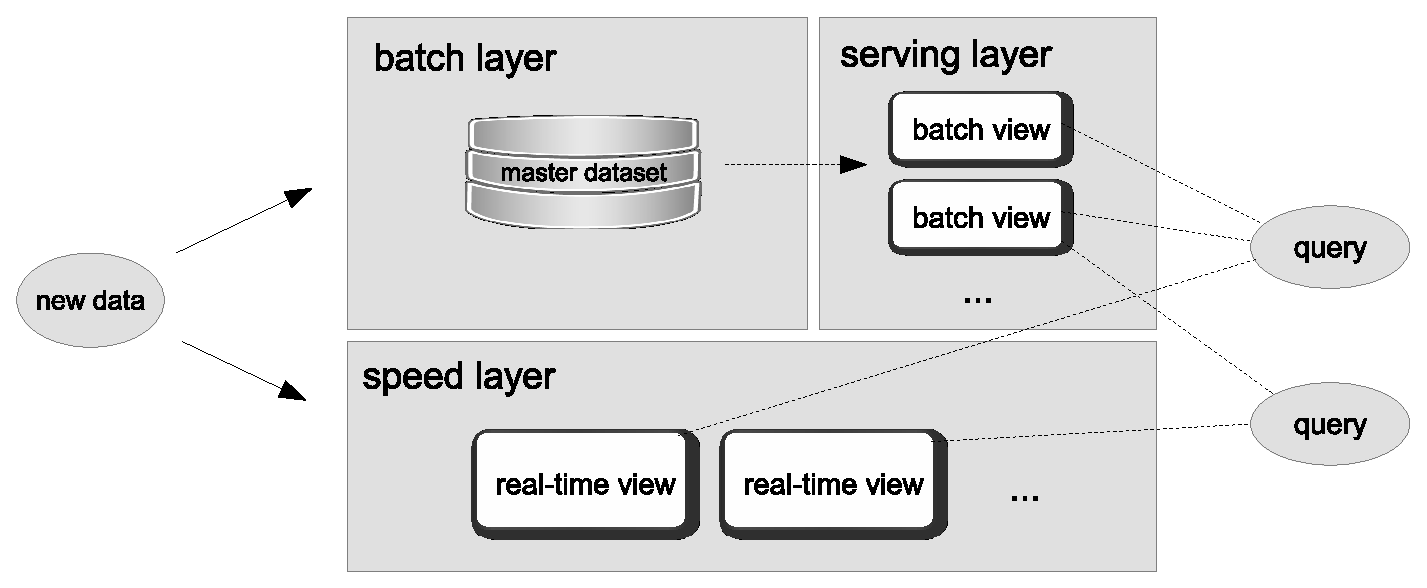
\includegraphics [width=1.0\textwidth]{images/LambdaArchitecture}
  \caption{General structure of the Lambda architecture. Batch and sevring layer are responsible for batch views, speed layer provides real-time views. To answer query system merges data from both types of views.}
  \label{fig:lambda_architecture}
\end{figure}

After the batch layer has precomputed views, it places them into the \textit{serving layer}\mnote{serving layer}.
The serving layer is responsible for storage of batch views.
It also creates indices on those views and provides interfaces to get particular data records from them.

Batch layer starts then computations again, considering now data, that has come during the last batch processing.
This loop goes on infinitely.
Batch processing always starts again from scratch using all available data.
When the batch layer stores computed views into the serving layer, it discards old ones.

Batch computations, although easy and efficient, take long time to be done.
This cannot be underestimated, because on the BigData scale computations can last hours even if we setup cluster of thousends of machines.
%In website example, assume our system has already been working for a year.
%It has then about 800 millions of posts.
%If we have a cluster of 100 machines, each has then to perform map-function 8 millions times.
%If one execution of map-function takes 1 milisecond, it leads to 2.2 hours of total computations.
%And we have not even counted reduce-phase.

As long as batch computations take much time, views are always outdated for several hours.
During this time new data arrives to the system, and it must be also counted in query answers.
This is not possible to solve using only batch processing.
Therefore, another approach is to apply.

To overcome delay of batch computations the Lambda architecture has additional component - the \textit{speed layer}\mnote{speed layer}.
It also computes views, but in incremental fashion.
We call them \textit{real-time views} \mnote{real-time view}.
As new data arrives, the speed layer updates incrementally real-time views.
Hence, they always has information from data, gathered during current batch processing.

Finally, to answer queries system uses both batch and real-time views.
Batch views contain result of the last batch processing.
Real-time views provide infromation from data, gathered after the beginning of the current batch processing.
Merging both types of views, system produces accurate and actual answers to the queries.
\section{Batch Layer}

The batch layer is the heart of the Lambda architecture.
It is the place where all ever gathered data resides and being processed.
The batch layer executes two main tasks: storing of data arriving from outer sources, and processing of that data to create batch views, used for the low-latency query answering.
The first issue requires usage of a storage system that provides fast appending, efficient batch reads, and no random reads/writes of data.
Computation of batch views demands application of distributed efficient batch processing algorithms as for example MapReduce.

\subsection{Data Model}

The batch layer requires usage of a specific data model to make the Lambda architecture scalable, highly efficient and fault-tolerant.
This data model is based upon four main notions.
\textit{Information} - the whole knowledge, that system holds.
\textit{Data} - collecting notion for records, strings, values, etc., kept in the system, so that they cannot be derived from any other data.
\textit{Query} - a question that is asked to the system, and demands a piece of information that answers it.
\textit{View} - a data structure that holds information directly useful for answering query.

\mnote{Raw data}
To answer as much different queries as possible, the batch layer stores only \textit{raw data}.
It is possible to derive from it data, particularly relevant for query, but not vice versa.
This is important, because the system does not know in advance all queries it will have to answer in the feature.
The more basic is the data, the more information can be possibly deduced from it.

In the current context, unstructured data is always better than normalized, because it is rawer.
As an example, let us consider the system, that stores users' search of a geographic location.
Suppose that system stores all those queries for further analytics.
If it saves them normalized, or in other words parsed and mapped to a known geographic location, it can for certain queries save nothing or NULL value, because algorithm cannot execute correct mapping.
In other case, when the system stores raw string, that user typed, it can later on have this data properly parsed, if parsing and mapping algorithms are improved.
This example shows, that unstructured raw data is preferred to store in the batch layer.

\mnote{Data immutability}
The batch layer does not allow modification or deletion of data, what is called \textit{immutability}.
It only allows appending new records.
This property gives two crucial advantages.
Immutability dramatically simplifies complexity of the storage mechanisms.
This is because maintenance of modifications in the distributed environment is not an easy task.
To successfully update a record, the system must perform it for all replications, provide locks and prohibit simultaneous updates.
It has to maintain versions of the same record for different users.
Absence of all these and many other requirements saves from much of complexity.
The system is easier to understand, repair and improve.
It is much safer from programming mistakes and consequent errors.

\mnote{Human fault-tolerance}
Another advantage of immutability is that mistakes in algorithms cannot corrupt data anymore.
This property is called \textit{human fault-tolerance}, and it is very important, because programmers always do mistakes.
As a result, it is possible, that wrong code can incorrectly update or delete data.
When data is immutable, programmers' mistakes can only append wrong data to the dataset.
This can be later repaired by administrator, but all proper data is always safe.

Immutability leads to high growth of data volume, because everything last stored basically forever.
This is, however, not a problem, because, as we discuss later on in this chapter, the batch layer is purely distributed and scalable.
It allows increasing capacity of its data store to any extent, adding new machines at any time.

Immutability requires completely different data model, comparing to relational databases, that manipulate tuples of complex objects altogether.
In contrast, the batch layer stores each attribute of a logical tuple separately.
Each value has the timestamp of addition moment. 
Such technique allows having the whole history of logical updates of all records.
The actual value is the one with the oldest timestamp.

\mnote{Eternal truthfulness of data}
Immutability gives one more important property of data, stored in the batch layer, namely \textit{eternal truthfulness of data}.
When new record is added, no matter is it a new piece of data or update of an old data, it represents true information in that particular moment in time.
This never becomes false, because it describes event or state of the world that is an occurred fact.
This property implies that the batch layer not only stores data, describing the state of the system, but also the history of its state changes.

\mnote{Master dataset}
Having defined the main properties of data, we can introduce the notion of the \textit{master dataset}.
The master dataset is the main storage, where all the data that ever arrived to the system resides.
The batch layer is responsible for its maintenance.
If there is a fault of the master dataset - all data can be lost.
And data is of the most importance in this context.
Therefore, the master dataset must be carefully designed, set up and protected.
It must be saved from all types of failures, e.g. software, hardware or human.
The master dataset is logically a large list of records.
When new piece of data arrives into the system, the batch layer appends it to the master dataset.
The more exact description of how the master dataset can look like will be discussed later on in this chapter.

\begin{figure}[h]
  \centering
  
\includegraphics [width=0.8\textwidth]{images/MasterDatasetExample}
  \caption{An example of the list of records in the master dataset.}
  \label{fig:MasterDatasetExample}
\end{figure}

On the Figure~\ref{fig:MasterDatasetExample} there is an example of the list of records of the master dataset.
The 5th and 6th records are updates of the 1st and 2nd, respectively.
They are in the same list, but the current version is defined by the last timestamp.
This model implies, that the whole history of updates is available at any time in the future. 

\mnote{Fact-based model}
In contrast to relational databases, data in the master dataset is stored using a so called \textit{fact-based model}.
It supposes that all the data is divided into simple units called facts.
Fact has several properties.
It is timestamped on addition to the master dataset.
Fact cannot be divided to a smaller units, it is already atomic.
Fact is identifiable in the sense that any two facts in the dataset must be distinguishable.

Fact-based model offers several important advantages.
It allows to make queries to a state of the dataset at any time in its history, because each piece of data (fact) is timestamped and immutable, or, in other words, eternally true.
It provides human-fault tolerance, as long as facts are immutable, and if a fact is added mistakenly, administrator can delete it.
If any of attributes of a complex object are absent, it is not necessary to store any NULL values, because data is stored in atomic facts.
Data can be stored in an unstructured denormalized form, because it is not queried directly from the master dataset, but from batch views of the serving layer, discussed later on.

\mnote{Graph schema}
To unite facts into related data there are so called \textit{graph schemas}.
Graph schema is a graph that describes the structure of a fact-based model.
It defines relations between entities similarly as entity-relationship model does for relational databases.
Graph schema consists of three elements: nodes, edges and properties.
Nodes are entities representing particular objects of a describable system.
Edges define relationships that connect nodes into the specific structure.
Properties provide information associated with nodes.

\begin{figure}[h]
  \centering
  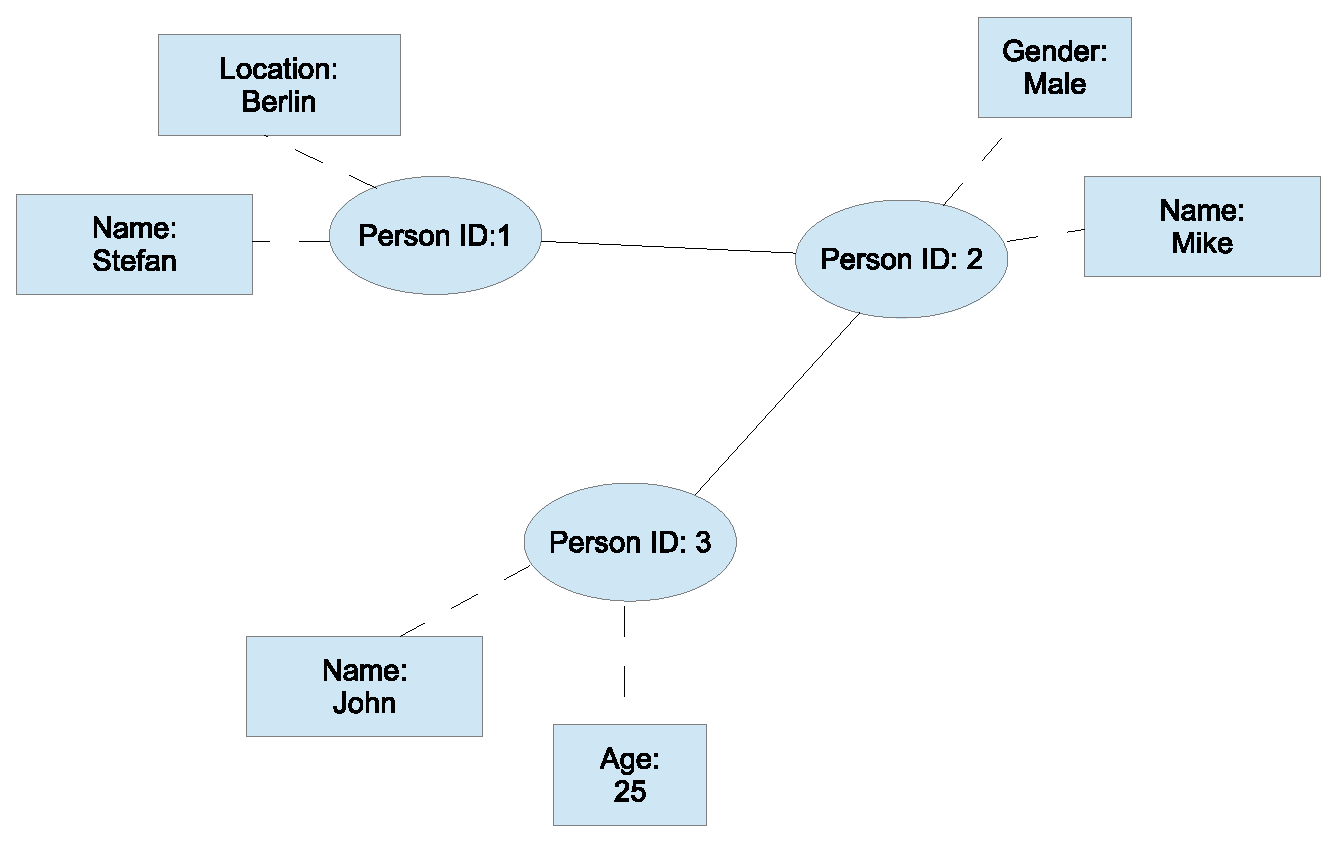
\includegraphics [width=0.8\textwidth]{images/GraphSchema}
  \caption{An example of graph schema.}
  \label{fig:GraphSchema}
\end{figure}

Figure~\ref{fig:GraphSchema} shows an example of a graph schema for a simple data model.
Entities are represented using ovals.
They are persons in this case.
Users are connected with their properties via dashed lines.
Lines between entities are edges.

\mnote{Serialization frameworks}
To save developers from detailed implementation of graph schema every time, and from possibility to do mistakes during this process, there are so called \textit{serialization frameworks}.
They provide a useful tool that generates all needed code, having described schema of the dataset in a specific descriptive language.
Serialization frameworks require only description of key notions, e.g. nodes, edges and properties.
They enforce then generation of all additional data fields and proper structure and data types for defined elements, as for example timestamps.  
Examples of serialization frameworks are Avro \ref{subs:avro} and Thrift \ref{subs:thrift}.

\subsection{Data Storage}

Physical data storage of the master dataset is another important issue.
In the big data context it is not possible to store all the data on one server.
Hence, distributed solution, that provides easy access, scalability and fault-tolerance, is required. 

\mnote{Requirements}
To understand requirements to the data storage, it is important to understand how data is going to be written and read.
Two main actions, it must support, are appending of new records and a bulk read for batch processing.
Immutability of data and continual appending demand, that high growth of the size of the master dataset must be easily affordable and maintainable.
Bulk reads require ability to access data in a parallel fashion.
There is no need for random writes or reads, what simplifies things dramatically.
Another important issue that the master dataset must allow to access only useful (for particular computations) parts of data.
This property is called \textit{vertical partitioning}.
The last requirement is that the master dataset must provide flexible way to store data compressed.

\mnote{Usage of HDFS}
There are many solutions that fulfil all described properties, starting from distributed file systems and finishing with distributed database systems. 
We choose the \textit{Hadoop Distributed File System} (HDFS), that we describe later on in all details \ref{subs:HDFS}.
Briefly, its main properties are: complete distributiveness that allows addition of as many new nodes as required, fault-tolerance via replication of data, high throughput via parallel access, tight connection with Hadoop MapReduce, simple access to the tree-structured file data.
HDFS fulfils all requirements that were stated for the master dataset storage system.

As long as HDFS stores data in the tree of files and folders, the way of applying it for the master dataset is straightforward.
All the data of the master dataset is then stored in the common folder.
Each piece of data, containing possible a set of records, is stored in a separate file that is automatically replicated.
There is also a necessity to fuse several small files into one big file periodically to avoid fragmentation and to increase batch access throughput.

An example of abstraction of the access to files and directories, that can be used to simplify access to HDFS, and to avoid use of a low-level HDFS API, is a \textit{Pail}.
Pail is a Java library, that allows working with HDFS in a more object-oriented way.
It makes code shorter an easier to read, and saves from many standard mistakes, that occur working with HDFS directly.

\subsection{Computation of Batch Views}

Answering particular query is often unreasonably expensive or even infeasible in the real time.
This is because amount of available data is huge, and because this data is raw. 
Moreover, query answer demands usually a piece of information that is far away from what raw data describes.
It requires often execution of complex algorithms on the whole dataset.
In the BigData context that can mean hours of processing, while low-latency response is typically a condition.

To solve this issue the batch layer precomputes batch views in advance.
Batch views contain derived data that is a result of execution of specific algorithms and aggregations on the whole dataset.
They help in answering particular queries.
The batch layer creates batch views in advance, so that they are ready for low-latency response in the query time.

The batch layer computes batch views in the infinite loop.
After completion of data processing, it starts from the beginning.
Processing of all the data and creating batch views is a long operation.
It can take hours and even days to be done.
As a result batch views are always out-of-date.
This is, however, can be considered as a deep analysis of data that connect pieces together to produce intelligent inference.
To overcome an issue of a long time processing, the Lambda architecture introduces the speed layer that we discuss in details later on in this chapter.

The batch layer executes specific functions on the master dataset that result in batch views.
These batch views store data that is easy to use to answer particular queries on the fly.
But it is important to mention, that this is not exact values that satisfy clients queries.
Rather, batch views hold data that can be on the fly used by the serving layer.
Storing of endpoint values would be in many cases way too expensive or even infeasible.
%Figure~ [add figure] shows this approach.

\mnote{Recomputation and incremental algorithms}
There are two approaches to compute batch views: to recompute them from scratch, and to make incremental updates.
Both of them have advantages and disadvantages that are the consequence of three properties: performance, human fault-tolerance, and generality of the algorithm.
Performance is usually much higher for incremental algorithms to compute batch views, because they simple do not have to process the whole master dataset, but only new data after previous processing.
But batch views has to be designed in a more complex way to allow incremental updates, what makes them usually larger, and slower to update.
Human fault-tolerance is inherent for the recomputational model.
If there is a mistake in building of batch views, it requires only removing that bug and deploying new code.
After next batch processing batch views will be properly created.
In contrast, for incremental method, it can be hard to find and correct results of mistakes in the algorithm.
It requires repairing of batch views, what is not an easy task in many cases.
Generality of the algorithm is a standard property of recomputational model.
Computations are simple and easy to tune, if query needs are changed.
Incremental algorithms are often approximated, what leads to a possible with some probability error in answering query.
They also move usually the part of computations to the querying time, what makes latency of the system's response higher.
As a result, it is strongly recommended to use recomputational algorithms.

\mnote{Application of Hadoop MapReduce}
Computation of batch views is an inherently distributed operation.
Developer does not have to think about multithreading issues.
He only writes simple one-threaded code, that is distributed then automatically in the cluster.
MapReduce is a perfect example of batch processing.
We have already discussed MapReduce programming paradigm in details in the Section~\ref{sec:mapreduce}.
Framework Apache Hadoop, based on HDFS, provides a powerful implementation of the MapReduce.
It is available for free as an open source product, and requires from developer only an implementation of \lstinline{map} and \lstinline{reduce} functions, what makes batch processing easy to implement in the real system.
\section{Serving Layer}

The serving layer is the end point in the approach of batch computations.
It provides low-latency answers to the clients' queries from the results of batch processing of the master dataset.
The serving layer has two main responsibilities: storing of the batch views, and creation of indexes for the fast access to those views.
The first issue requires usage of a storage system that fulfils several specific requirements, as for example fast batch writes and fast random reads. 
Creation of indexes on batch views demands from the serving layer to tackle such problems as for instance denormalization of data.

Each time the batch layer finishes computation of batch views, it stores them into the serving layer, discarding the old ones.
The speed layer recomputes then its indexes.
Problems with batch views or indexes, as for example inconsistency or corruption of data, are only temporal.
They are repaired after the next batch processing.

\mnote{General requirements}
The serving layer has two main metrics of efficiency: throughput and latency.
Throughput implies the number of queries that can be done in the time unit.
Latency is the time to execute one particular query.
To satisfy both of these properties it is important to design indexes of batch views in a specific way.
For example, in case of storing key-value data, data associated with the key must be collocated on the same machine and stored sequentially.
This makes reading much faster (especially in case of HDD usage), because requires only one disk seek and following sequential read.
Generally, indexes must require access to as few as possible machines for retrieving data, needed for answering query.

\mnote{Denormalization of data}
The serving layer allows denormalization of data in the batch views on indexes creation.
This is opposite to the master dataset, where it is possible to keep completely normalized data.
The batch layer does not have to provide low-latency response, and can process such data without any penalty, doing joins or any other data linking.
The serving layer has to return data fast, what imposes a need to make access to indexes as efficient as possible.
Denormalization of data saves from expensive joins.
This makes request time much smaller.

Denormalization leads usually to a redundancy of data.
It also can result in inconsistency of a repeated data pieces, especially when the system becomes complex.
This is, nevertheless, not a problem because of two things.
Firstly, space is not an issue in the serving layer, as long as distributed storage is used, and any number of machines can be added any time.
Secondly, even if there is an inconsistency in data in prepared indexes, it is only temporal, and will be repaired after the next update of batch views.

\mnote{Database requirements}
Database system, that the serving layer uses, must fulfil several requirements.
First of all, it must provide batch writes.
The batch layer recomputes batch views from scratch, and override old ones with newly computed.
It must be possible to write them in a batch fashion efficiently.
The second required property is scalability that is the database system must be essentially distributed.
It must allow addition of as many new machines as needed in case of growth of space requirements.
The third point is ability to make fast random reeds.
This is highly important for a final low-latency query response.
Specifically, fast random reeds of data in prepared indexes gives required efficiency.
The last issue is fault-tolerance, what is a standard property for the Lambda architecture.
It must be provided for the serving layer via distributed database system with replications.

\mnote{Example of a storage system}
An example of a storage system that can be used for the speed layer is ElephantDB \cite{ElephantDB, Macbeth2013}.
The main properties of ElephantDB is that it is a key-value store, that is simple, easy to use, distributed, and open source.
It fulfils all requirements of the speed layer storage system.
Specifically, it allows making batch writings, for example as a result of MapReduce computations.
Also, it provides fast read-only random reads.
It does not support random writes, what makes it so simple and almost saves from bugs.
\section{Speed layer}

To overcome delay of the batch processing the Lambda architecture has the speed layer.
It applies the real-time incremental processing to arriving data.
The speed layer has higher complexity than the batch layer, because of the incremental nature of applied algorithms.
It provides usually approximated results, because algorithms, used for online processing, are often approximated.

The speed layer computes real-time views, that are similar to batch views in the sense, that they store data useful for fast answering queries.
Real-time views contain data, observed during ongoing batch processing in the batch layer.
The speed layer also prepares indexes on those views, that allow to answer queries ``on the fly''.

\subsection{Computation of real-time views}

To compute real-time views, one could consider the same approach as for batch views, but use only new data for computations.
This would simulate batch processing on the much smaller scale.
Nevertheless, if we want to achieve latency of miliseconds, such approach is not going to work.
Batch processing even on the scale of several gigabytes is not possible to do in miliseconds.

To solve this issue there is a completely different approach.
Real-time views are not considered as a function of a recent data, that has arrived during current batch processing.
Instead, they are the result of the function of a new data, that just came, and of their previous state.
Basically, it is an incremental update with a small piece of data, everytime it arrives.
This normally leads to only approximated answers to the queries, provided by real-time views.
But this is again not a problem, because error does not accumulate for too long.

\subsection{Data storage}

Speed layer must obey low-latency requirement, and must allow application complex incemental algorithms.
Having such demands, storing of real-time views requires several properties to be fulfiled: ability to make random reads and writes, scalability and fault-tolerance.
Ability to make random reads is particularly important to make answering queries fast.
Ability to make random writes is necessary, because of the need to apply incremental algorithms, that always demand this property.
Real-time views must be scalable, because amount of data to process can still be of a huge size.
That means, that distribtuion to many machines must be supported.
Fault-tolerance is as usual must be provided via replications of data in the real-time views.

There are many storage systems, that fulfil these properties.
They are usually called \textit{NoSQL databases}\mnote{NoSQL database}.
They store data using different data models than relational databases.
We have already briefly discussed one of such system, namely ElephantDB, that was useful for storing batch views in the serving layer.
One can choose specific database, that fulfils his or her requirements to data representation.
Sometimes batch and real-time views has the same data format.
But it is not always the case, because it is not always easy to execute the same function in the batch and in the incremental way.
Also, as long as real-time views have to be updated incrementally, they have more complex data structure.
Because of those factors, it often happens, that real-time views represent data differently, than batch views.

\subsection{Issues of incremental computations}

We have already discussed the difference between incremental and recomputation algorithms.
Batch computations imply, that computations of a specific function is executed on the whole dataset.
This is usually easy to program, even though can take much time.
In case of incremental computations, building of real-time view is going continuously.
It is usually more efficient, but can lead to accumulation of error, especially if programming mistake takes place.

The important aspect to discuss it a relation of incremental computations and a so called CAP theorem.
The CAP theorem states, that consistency and availability are not possible simultanously to achieve, when data is partitioned.
The meaning of the CAP theorem is that it is possible to make the system completely available, but it can sometimes return not yet actual data, or it is possible to make it truly consistent, but it can sometimes provide now response for a request, because data is not yet propogated to partitions.

There several ways of how to design the system, so that it provides consistency or availability completely, or has a tradeoff between them.
System is fully consistent, if it updates all replicas of a piece of data at once, and only then allow to access this data.
It is fully available, if it stores an update as a new temporal record, and then tries to merge it with the real data in the system.
This can take time, and reading of that data can return old values.

To achieve a tradeoff there so called \textit{conflict-free replicated datatypes} (CRDTs).
They provide eventual consistency working in a distributed fashion.
For example the G-Counter allows to maintain a counter, that allows only incrementation.
It stores different versions of an integer counters in different replicas, and the merge them to provide correct results.
There is unfortunately no way to aboid this complexity, and to make the system fully consistent and available at once.

\subsection{Expiration period of real-time views}

Real-time views, though more complex than batch views, but have only transient nature.
They are discarded every time, when batch layer completes processing of batch views.
Batch views then contain all information, that real-time views gathered during the last batch processing. 
Such temporal nature of real-time views saves from accumulation of error, and leads to eventual accuracy of query answering.

The simplest solution of discarding old real-time views is to set expiration time or period.
But it suffers from unstability of the duration of batch processing, that can vary every time.
Because of that, more robust, generic solution were proposed.

Let us consider a new information system, that does not have yet any data.
On the first run of batch processing the master dataset is empty.
But it still takes time, let say 10 minutes, because of overhead for creation of empty views, indexes, and so forth.
The speed layer gathers during this first batch processing data, and to its end has already real-time views, containing data, processed during this 10 minutes.

When the second start of batch computations runs, it consider the first 10 minutes of data, that resides now in the master dataset, for processing.
The speed layer continues to update real-time views.
Let's say the second batch processing takes 15 minutes.
To its end batch views have the reflection of the first 10 minutes.
Real-time views reflect all 25 minutes of system's life.
Now the part of them, that was built during th first 10 minutes can be discarded.

When the third batch processing starts, it considers data gathered during 25 minutes.
The online processing in the speed layer has updates now views, that has 15 minutes of processed data, gathered during the second batch processing.
Let's say the batch processing takes 18 minutes now.
When it finishes, batch views reflect the first 25 minutes of data, whereas real-time views reflect 33 minutes of data, starting after 10 minutes of the system's functioning.
Now real-time views must leave only reflection of the last 18 minutes of arriving data.

To make it possible, two sets of real-time views must be maintained.
The speed layer then switch between them after each finish of the batch processing.
Each set of real-time views store them results of processing during two consecutive batch runs.
This can look redundant and expensive, but is actually not, because real-time views store only small data, gathered during short time.

\section{Requirements compliance}

Robust
Fault-tolerant
Responses with low-latency
Scalable
Generic
Extensible
Allows ad hoc queries
Requires minimal maintenance
Debuggable
\section{Distributivity}

I'm not sure about this section